

\section{Admissible Term Structures}
\label{sec:admissible-curve}
The previous problematic is also present  for some other derivative product such
as : 
\begin{itemize}
\item Corporate bond yield curve
\item Discounting curve based on OIS
\item Forward curve based on fixed-vs-Ibor-floating IRS
\end{itemize}
All this term-structure construction consist in finding a function $T \lra P(t_0,T)$
given a small number market quotes $S_1,...,S_n$. 

\quad Indeed, We have to rely on interpolation/calibration schemes to construct the
curve for the  missing maturities.\\
\quad This will lead us to define what will be understood by a good yield curve
construction.\\

\subsection{Notation}
\label{sec:notation}
First Let's de fine some notations in order to be concise :
\begin{description}
\item[n] The number of maturities
\item[$\mathbf{t_0}$] The cotation date
\item[S] $=(S_1,S_2,\dots,S_n)$ The set of market quotes at $t_0$
\item[T] $=(T_1,\dots,T_n)$ the corresponding set of increasing maturities 
\item[t] $=(t_1,\dots,t_{p_n})$ payment time grid
\end{description}

The payement time grid are arranged as : $\forall i \in 1 \dots n\ T_i=t_{p_i}$
\begin{figure}[H]
  \centering
  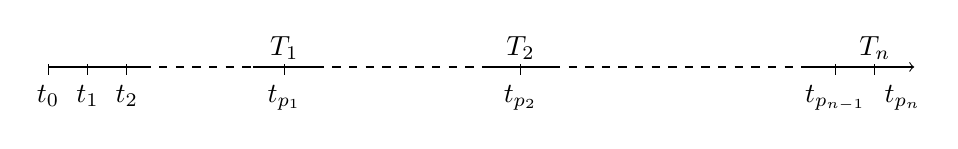
\begin{tikzpicture}
    \draw  (0 cm,1pt) -- (0 cm, -3pt) node[anchor=north] {$t_0$};
    \draw  (0.5 cm,1pt) -- (0.5 cm, -3pt) node[anchor=north] {$t_1$};
    \draw  (1 cm,1pt) -- (1 cm, -3pt) node[anchor=north] {$t_2$};
    \draw  (3 cm,1pt) -- (3 cm, -3pt) node[anchor=north] {$t_{p_1}$};
    \draw  (3 cm,1pt) -- (3 cm, -3pt) node[above=2pt] {$T_1$};
    \draw  (6 cm,1pt) -- (6 cm, -3pt) node[anchor=north] {$t_{p_2}$};
    \draw  (6 cm,1pt) -- (6 cm, -3pt) node[above=2pt] {$T_2$};

    \draw  (10 cm,1pt) -- (10 cm, -3pt) node[anchor=north] {$t_{p_{n-1}}$};
    \draw  (10.5 cm,1pt) -- (10.5 cm, -3pt) node[below right] {$t_{p_{n}}$};
    \draw  (10.5 cm,1pt) -- (10.5 cm, -3pt) node[above=2pt] {$T_n$};

    \draw (0,0) -- (1.2,0);
    \draw[dashed] (1.2,0) -- (2.8,0);
    \draw (2.6,0) -- (3.4,0);
    \draw[dashed] (3.4,0) -- (5.8,0);
    \draw (5.6,0) -- (6.4,0);
    \draw[dashed]   (6.4,0) -- (9.6,0);
    \draw[->] (9.6,0) -- (11,0);

  \end{tikzpicture}
  \caption{Time grid }
  \label{fig:3}
\end{figure}

\subsection{Market fit condition}
\label{sec:market-fit-condition}
We assume first that this quotes can be presented in a linear form, which is the
case for the previous instruments presented :
\begin{assumption}[Linear representation of present values \cite{OTRATS}]
  \label{ass:1}
  Present values of products used in the curve construction process can be expressed as linear combination of some elementary quantities. Depending on the context, the latter can be either zero-coupon prices, discount factors, Libor or Euribor forward rates or CDS-implied survival probabilities.
\end{assumption}
\begin{example}[Credit curve based on CDS]
  From equation (\ref{eq:3}), by integration by parts we can get:
  \begin{eqnarray*}
    \label{eq:2}
    S_i \sum^{p_i}_{k=1}\delta_kP^D(t_0,t_k)Q(t_0,t_k) - (1 -
    R)P^D(t_0,T)Q(t_0,T) & \\
    + (1 - R)\int^{T_i}_{t_0}f^D(t_0,t)P^D(t_0,t)Q(t_0,t)dt & = 1 - R,\ i=1,\dots,n.
  \end{eqnarray*}
  where $f^D(t0, u)$ is the instantaneous forward (discount) rate associated with
  maturity date u and the . Therefore CDS can be written as a linear equation of
  {\it survival probability} ($Q(t_{p_i})$).
\end{example}

\sauta
This condition can be written more generally and more algebraically in this form :
The Term  structure function $T  \lra P(t_0,T)$ is  built from market  quotes of
standard product.


Let $P=(P^D(t_0,t_1),\dots,P^D(t_0,t_m))$  be the  vector of  the values  of the
curve $T \lra P(t_0,T)$ at the payment dates $t_1,\dots,t_{p_n}$: 

The  market fit  condition can  be restated  as a  rectangular system  of linear
equations :
\[
A \cdot P=B
\]

where :
\begin{description}
\item[P] =$(P(t_0,t_1),\dots,P(t_{0},t_{p_n}))'$ A vector of curve $T \lra P(t_0,T)$ at the
  payement time grid
\item[A] is a $n \times p_n$ matrix
\item[B] is a $n \times 1$ matrix with positive coefficients
\item A and B only depend on current market quotes S, on standard maturities T, on payment dates t and on products characteristics.
\end{description}

A lot of curves can satisfies the market, in order to get an admissible curve $T \lra P(t_0,T)$ have to fit some others
conditions. 

\subsection{Arbitrage-free conditions}
\label{sec:arbitr-free-cond}

\begin{de}[arbitrage-free condition]
  \label{def:2.1}
  A credit  curve is  said to be  arbitrage-free if the  curve corresponds  to a
  well-defined default distribution  function. In other words $P$  had to verify
  the following conditions :
  \begin{itemize}
  \item $P(t_0,t_0)=1$
  \item $T\longmapsto P(t_0,T)$ is non increasing function (i.e $\exists x,y, P(t_0,x)<P(t_0,y)\&x>y$)
  \end{itemize}
\end{de}

\begin{example}[NB]
  \label{arbitrage-free}
  If a credit  curve didn't satisfy the arbitrage free  condition, then there is
  some arbitrage opportunities in the market. 
\end{example}

Therefore we have  the following inequalities, called \green{\textit{Arbitrage-free
    inequalities}} :
\label{arbtr-free-inq}

\begin{center}
  \begin{align*}
    P(t_0,T_1) & \leq P(t_0,t_k) \leq 1 & \forall k \in 1,\dots,p_1 \\
    P(t_0,T_i) &\leq P(t_0,t_k) \leq P(t_0,T_{i-1}) & \forall k \in [p_{i-1}+1
    , p_i-1 ]\\
  \end{align*}
\end{center}

Admissible curve require also to be smooth :
\begin{de}[Smoothness condition]
  \label{def:2.2}
  A curve  is said to be  smooth if it  is differentiable and his  derivative is
  continuous.
\end{de}


\begin{rem}
  \begin{itemize}
  \item For example,  a credit  curve (\textit{CDS})  satisfies the  smoothness condition  if the
    associated default density function exists and is continuous.\\
  \item Also  an IR  curve  (\textit{OIS})  satisfies the  smoothness  condition if  the
    associated  instantaneous  forward  rates  exist  for  all  maturities  and  are
    continuous.
  \end{itemize}
\end{rem}

\sautb
In summary :
\begin{de}[Admissible Curve \cite{OTRATS}]
  Given a set of observed market quotes. A  curve is said to be admissible if it
  satisfies the following three constraints :
  \begin{itemize}
  \item The selected market quotes are perfectly reproduced by the curve.
  \item The curve is arbitrage-free in the sense of Definition \ref{def:2.1}.
  \item The curve satisfies the smoothness condition presented in Definition 
    \ref{def:2.2}.
  \end{itemize}
\end{de}

\subsection{The geometrical side of admissible curves}
\label{sec:geom-side-admiss}

\paragraph{}

\textit{Let denote by $\mathcal{C}$ the set of admissible Curves.}

\begin{prop}
  the set of admissible curves $\mathcal{C}$ is convex
\end{prop}

\begin{proof}
  Let  $P_1,P_2\in \mathcal{C}$  then  by the  Assumption \ref{ass:1},  $\exists
  A \in \mathcal{M}_{n,p_n}(\mathbb{R}),\ \exists B \in
  \mathcal{M}_{n,1}(\mathbb{R})$\footnote{Until we are working at one product at
    a time (CDS, OIS , $\dots$) the matrices $A,B$ are uniques for all admissible curves} that verifies :
  \begin{align*}
    A  P_1 &= B\\
    A P_2 &= B\\
  \end{align*}
  Let $\alpha  \in [0,1]$ then  : $\left(\alpha P_1  + (1 - \alpha)P_2\right)  A = B$  so $P=
  \alpha  P_1  +  (1-\alpha)P_2$  verifies the  Assumption  \ref{ass:1}.   $P$  is
  smooth(resp continuous)
  as far as $P_1,P_2$ are smooth(resp continuous). So $P \in \mathcal{C}$.
\end{proof}


All the  admissible curves are  bounded : $\forall  f \in \mathcal{C},\  0\leq f
\leq 1$.  One brave question is  to say if there  is min (resp max)  for the set
$\mathcal{C}$ ? . This will naturally lead us to study the \textit{compactness} of the set
$\mathcal{C}$ since it's already convex. 

\paragraph{}
Let's remind a theorem in compactness of function spaces :
\begin{thm}[Ascoli-Arzela]
  Let $(E,d)$ a compact metric space, and $(F,\delta)$ a full metric space.\\
  A subset \textit{A} of $\mathcal{C}(E,F)$ is relatively compact if and only if :
  \begin{enumerate}
  \item A is equicontinuous:
    \[
    \forall  x \in  E, \forall  \epsilon >  0 ,  \exists \eta  > 0  / \forall  f \in
    A,\forall y \in E, (d(x,y) \leq \eta ) \Lra (\delta(f(x),f(y)) < \epsilon)
    \]
  \item $\forall x \in E$, the set $A(x)=\left{ f(x),f \in A\right}$ is relatively
    compact.
  \end{enumerate}
\end{thm}


% \quad A.Cousin had demonstrate the following proposition :

% \subsection{Application on AIG CDS data spreads}
% \label{sec:application-aig-cds}

% \quad If the assumption arbitrage-free is not verified the previous results will not
% be relevant. Indeed we  see this phenomenon when we tried  to apply the previous
% bounds  over  the  data  provided  by  {\it AIG  (France)}.  We  note  that  the
% arbitrage-free inequalities where no longer verified. \\

% \begin{figure}[H]
%   \label{fig:5}
%   \centering
%   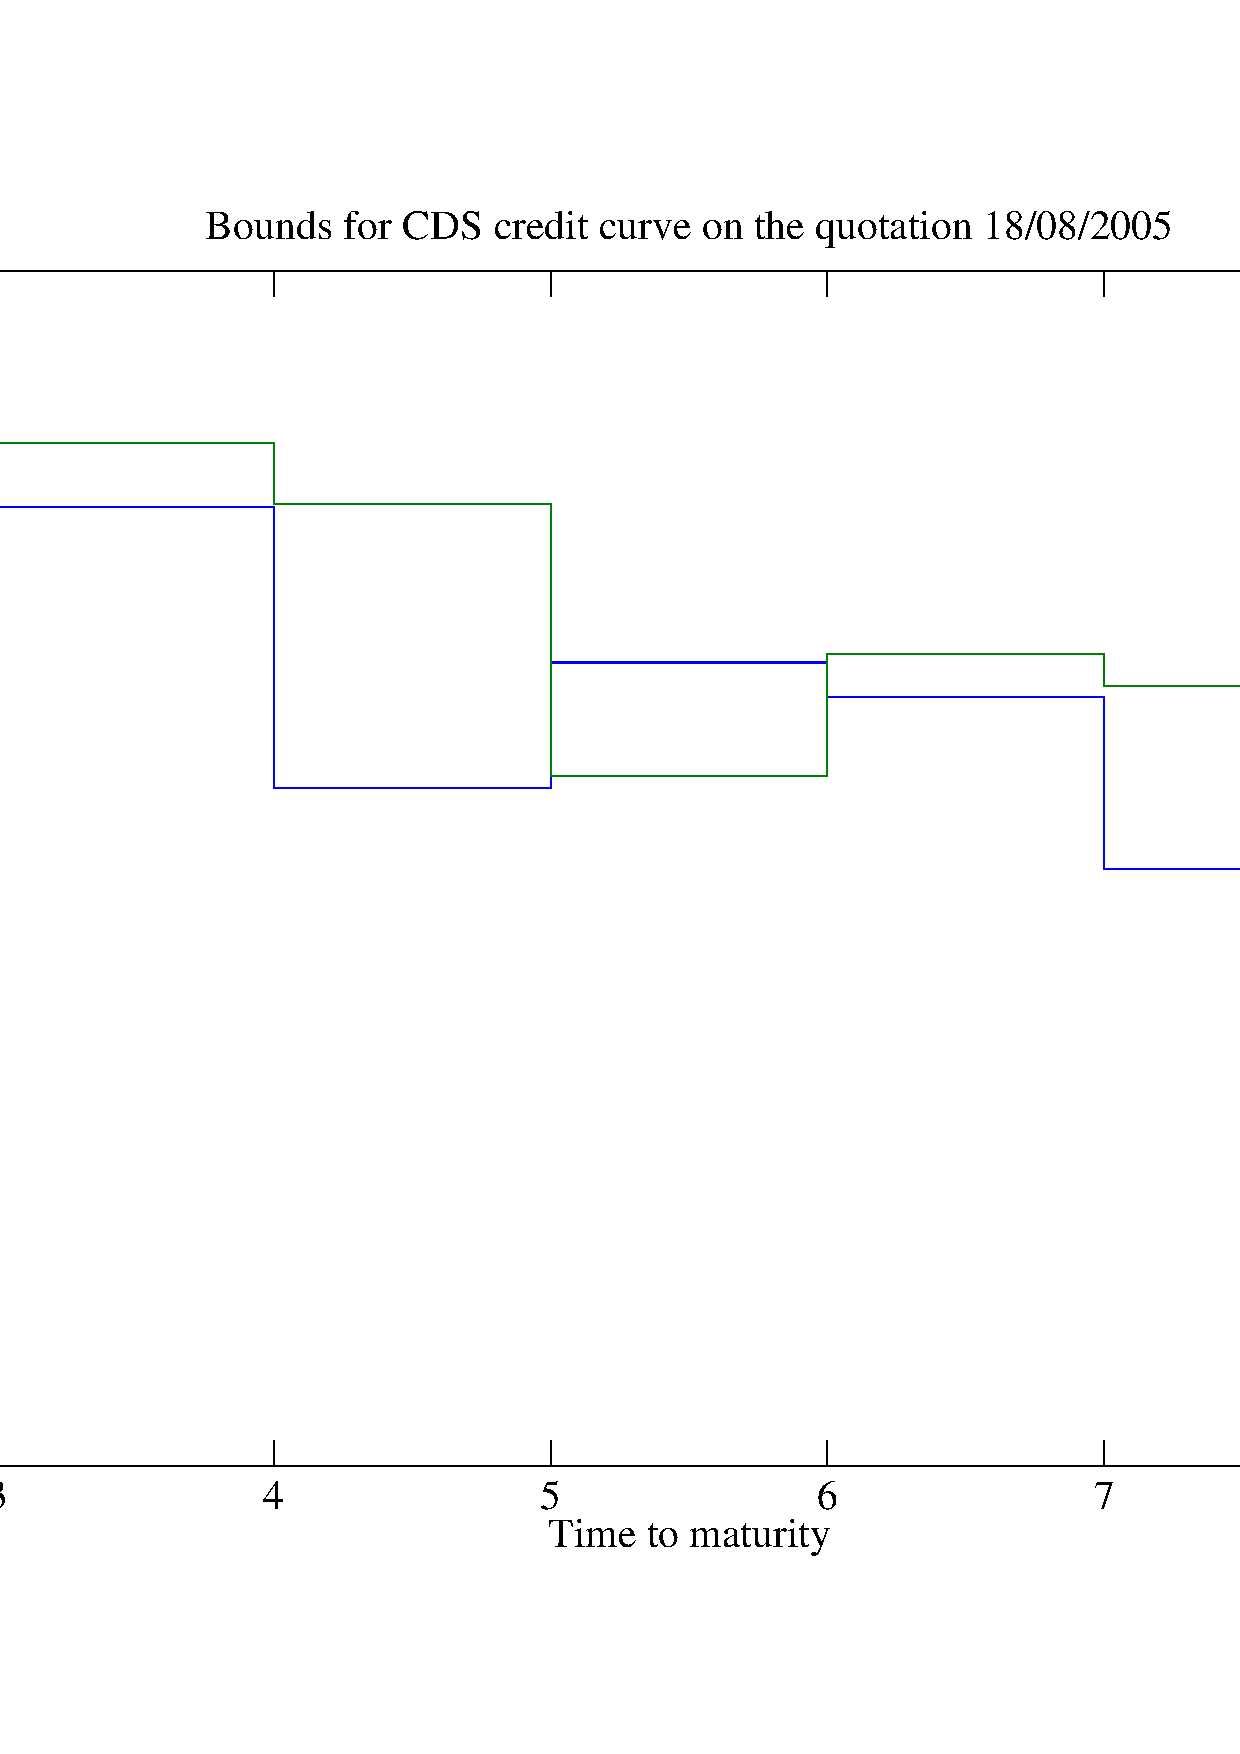
\includegraphics[width=0.7\textwidth]{cotation-18-08-2005.pdf}
%   \caption{Credit curve among 18/08/2005 -  28/09/2007}
% \end{figure}


% It   means    that   the    market   since   18/08/2005    contained   arbitrage
% opportunities.  Indeed  between  18/08/2005   -  28/09/2007  the  market  wasn't
% complete.

% \begin{figure}[H]
%   \centering
%   \includegraphics[width=0.8\textwidth]{cotation27-11-2007.pdf}
%   \caption{Credit curve since 28/09/2007 : here in 27/11/2007}
% \end{figure}


